\subsection{Consideraciones sobre los tests}

\begin{itemize}

\item {Los tests que implementamos para medir el rendimiento de los programas fueron implementados en C utlizando las instrucciones de assembler RDTSC para obtener el valor del Time Stamp Counter y CPUID para evitar que el código que queremos medir se realice con ejecución fuera de orden. Esta instrucción sincrónica, la usamos entonces, para serializar la ejecución del código.}

\item {El código consiste en 1000 ejecuciones seguidas de las distintas implementaciones de los filtros, obteniendo los resultados con la cantidad de ciclos que tardo cada una de ellas en una planilla de excel .svc .}

\item {Para evitar, en parte, el overhead, decidimos modificar las funciones run_[nombre_del_filtro] provistas por la cátedra, de modo que se comience a medir los ciclos justo antes de llamar a la funcion que aplica el filtro, sin contar las operaciones sobre los bmp que realiza antes y despues del llamado a esta. }

\begin{figure}[ht!]
\centering
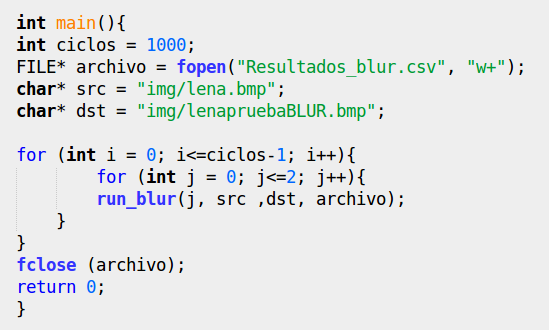
\includegraphics[width=90mm]{imagenes/resultados/codigoblur.png}
\caption{Código para testear rendimiento de Blur.}
\end{figure}

\begin{figure}[ht!]
\centering
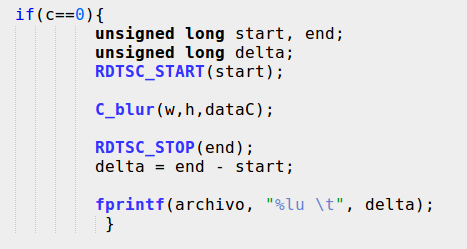
\includegraphics[width=90mm]{imagenes/resultados/codigoblur2.png}
\caption{Extracto de código modificado de run_blur en run.c.}
\end{figure}

\item {Como primera observación, el código no arrojaba los mismos resultados si realizamos 1000 iteraciones seguidas de la misma implementación en lugar de ir alternandolas. Es decir, si hacíamos 1000 ejecuciones de C, luego las 1000 de ASM1, y finalmente las 1000 de ASM2, las últimas ejecuciones del código, principalmente las de C, observamos que el tiempo que tarda en ejecutar cada iteración se vuelve menor, en parte probablemente al aprovechamiento de la cache. Para solucionar ésto, decidimos alternar la ejecución de las implementaciones, de manera que nuestro código ejecute 1 de C, 1 de ASM2, 1 de ASM2, y luego comenzar de nuevo hasta completar las 1000 iteraciones.}

\item {Una vez obtenidos los tiempos de cada iteración, usando las funciones que provee LibreCalc (Excel), calculamos la media de la muestra para cada implementación y su desvío estandar.}

\item {Para filtrar los outliers, decidimos calcular el rango determinado por la fórmula a continuación, de manera que aquellas mediciones fuera de rango, sean sacadas de la muestra. De esa manera calculamos un nuevo promedio con la "podada" de la muestra, y su nuevo desvío estandar.}

Rango aceptable para las mediciones: 
\[
(q_{1} - 3*IQR ;\ q_{3} + 3*IQR) ,\ con\ IQR = q_{3} - q_{2}
\]

\item {Para realizar las mediciones utilizamos una notebook sony VAIO con procesador Intel Core i5, 5.7gb de memoria RAM y s.o. Ubuntu 14.04 de 64bits.}

\end{itemize}


\subsection{Experimento 1}

Este primer experimento busca relacionar el rendimiento de las implementaciones de C, ASM1 y ASM2 de cada filtro, de manera general. Para ello, mostraremos en profundidad los resultados obtenidos por cada implementación para una imagen determinada, comparando con la versión no optimizada del compilador de C. (En este caso, lena.512x512.bmp, con value=0.5 en los casos del merge y hh=360, ss=0.2 y ll=0.1 en los casos del hsl.)

\begin{figure}[ht!]
\centering
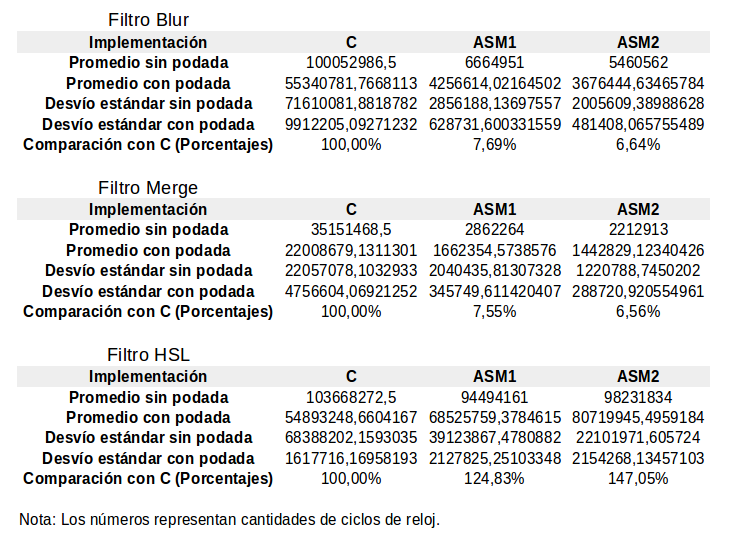
\includegraphics[width=150mm]{imagenes/resultados/tablacomparacion.png}
\caption{Tablas de Resultados para cada Implementación, 1000 iteraciones.}
\end{figure}

Como se puede notar en la tabla, para este caso, obtenemos los siguientes resultados con respecto al rendimiento de las implementaciones:

\begin{itemize}

\item { En el caso de Blur, la implementación ASM1 corre aproximadamente 13 veces más rápido que la de C, mientras que la de ASM2 corre 15 veces más rápido. Ésto es lógico pues en la segunda implementación se procesa de a 4 píxeles a la vez, mientras que en la primera se procesa de a 1 por vez, sin embargo, no es una diferencia demasiado notable, teniendo en cuenta el desvío estandar de la muestra podada. }
\item { En el caso de Merge, obtenemos aproximadamente las mismas relaciones con respecto a C. ASM1 funciona 13 veces más rápido que C, mientras que ASM2 15 veces más rápido. Ésto se debe a que al trabajar con enteros, en ASM2, nos ahorramos las conversiones a floats de los componentes, además de un paso de desempaquetado extra que no es necesario ya que podemos trabajar directamente con los words enteros. Sin embargo, al observar las imágenes resultantes, aparece una pequeña, y a nuestro criterio, aceptable pérdida de precisión. Como mucho, los componentes de la implementación en enteros varían en 1 con respecto a las otras.}
\item { Por último, en el caso de HSL, a diferencia de las anteriores, C le saca ventaja a las dos implementaciones de assembler. La de C tarda aproximadamente el 80\% de lo que tarda la de ASM1, y un 70\% de lo que tarda la de ASM2. Es decir, ASM2 es la de menor rendimiento. Existen diversos motivos que posibilitaron este resultado:
	\begin{itemize}
	\item {En principio, para las llamadas a rgbTOhsl y viceversa, fue necesario tener un vector auxiliar donde guardar los resultados de dichas funciones, haciendo que se necesite un nivel alto de accesos a memoria.}
	\item {Además, la complejidad de las conversiones, en caso de ASM2, complejizaron el algoritmo, pues en C la secuencia de ifs se resuelve de manera más rápida que de la forma en que esta implementada usando instrucciones de SIMD. En assembler, y con esta implementación, es necesario corroborar todas las condiciones de los ifs anidados, y actualizar los valores en caso de que se cumplan, a diferencia de C, en donde una vez que se cumpla una de ellas no es necesario revisar las demás. Además, para complejizar aún más, se utilizan en varias ocasiones máscaras, que se traducen en más accesos a memoria, e instrucciones de SHUFFLE para facilitar la manipulacion del orden de los componentes durante la conversión. }
	\item {Otro punto a tener en cuenta, es por ejemplo, la manera en que están implementadas las funciones fabs y fmod en C, pues en nuestra implementación fabs corresponde a un acceso a memoria y la aplicación de una máscara que modifica el bit de signo, mientras que para calcular fmod es necesario una serie de operaciones, incluida una conversión de float a entero. Ésto hace probable que éstas, y algunas otras funciones en C puedan estar implementadas más eficientemente.}
	\item {Por último, y no menos importante, las llamadas reiterativas a C en ASM1 producen overhead.}
	\end{itemize}
	}
\end{itemize}	

El siguiente gráfico muestra de manera más clara las relaciones comentadas anteriormente entre las distintas implementaciones:

\begin{figure}[ht!]
\centering
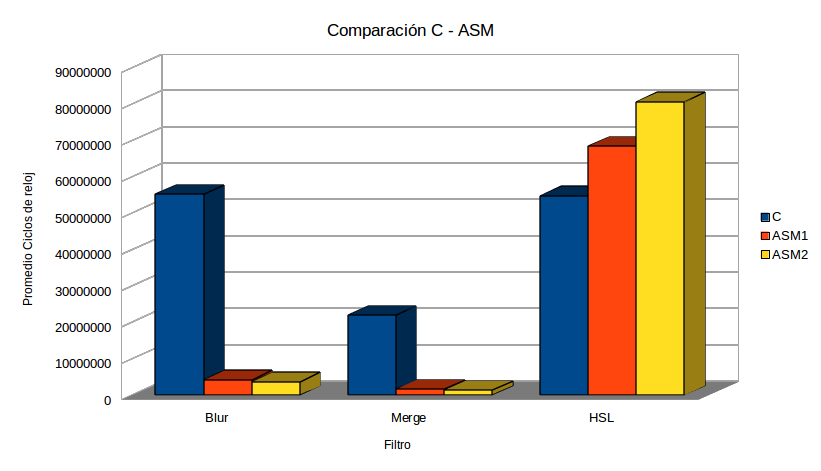
\includegraphics[width=120mm]{imagenes/resultados/graficocomparacion.png}
\caption{Gráfico de Barras, Comparación C-ASM, Experimento 1.}
\end{figure}

\newpage


\subsection{Experimento 2}

En este experimento comparamos el rendimiento de las implementaciones con respecto a los diferentes tamaños de entrada. Para ello, modificamos la imagen lena.bmp y medimos los tiempos de ejecución para cada tamaño. Decidimos hacerlo solo para Blur y Merge para ganar claridad en el gráfico, ya que los valores de los tiempos promedio de HSL difieren bastante con los de Blur y Merge.

\begin{figure}[ht!]
\centering
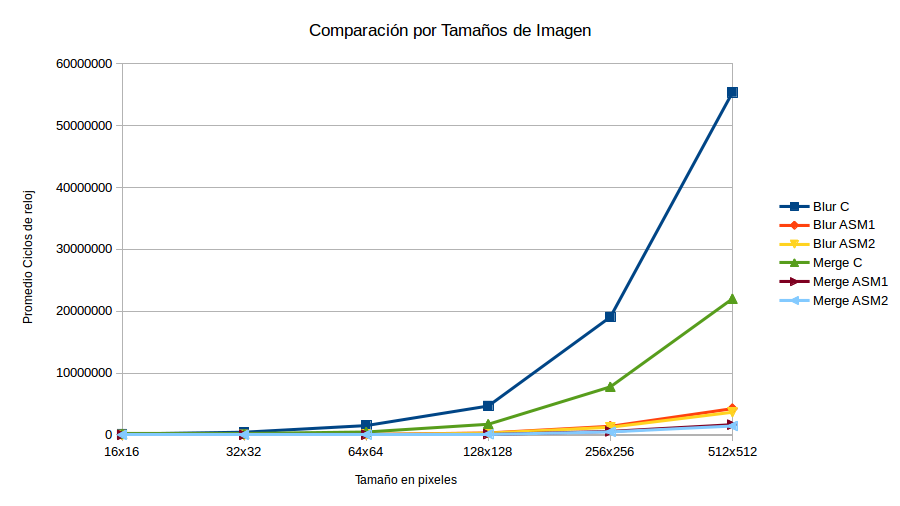
\includegraphics[width=150mm]{imagenes/resultados/graficotamanio.png}
\caption{Gráfico de Líneas, Experimento 2.}
\end{figure}

Como resultado importante, vemos que al aumentar el tamaño de la entrada (en cada punto se cuadriplica el tamaño de la imagen), la version de C crece mucho más rápido que la de ASM, es decir, la cantidad de ciclos que le toma a C procesar imágenes cada vez más grandes aumenta más velozmente que lo que le lleva a las funciones en asm. De manera que cuanto mayor es el tamaño de la imagen, más notoria es la ventaja de los programas realizados en asm. 


\subsection{Experimento 3}

En este experimento, comparamos cada implementación de los filtros contra las distintas optimizaciones posibles del compilador gcc para la version implementada en C.

\begin{figure}[ht!]
\centering
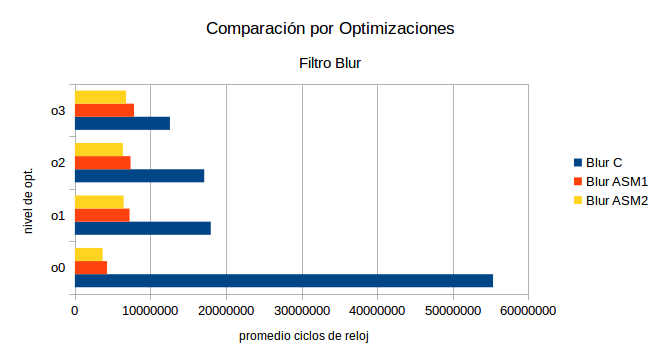
\includegraphics[width=125mm]{imagenes/resultados/grafico-opt-blur.png}
\caption{Filtro Blur, Experimento 3.}
\end{figure}

Observamos que la eficacia de los programas implementados en C depende directamente del grado de optimización con el que lo compilamos. En los casos de Blur y Merge, aún comparando con la optimizacion 3, las versiones en assembler andan más rápido que las de C, mientras que HSL de C supera  a las de ASM con más amplia claridad a medida que aumentamos el nivel de optimizacion.

\begin{figure}[ht!]
\centering
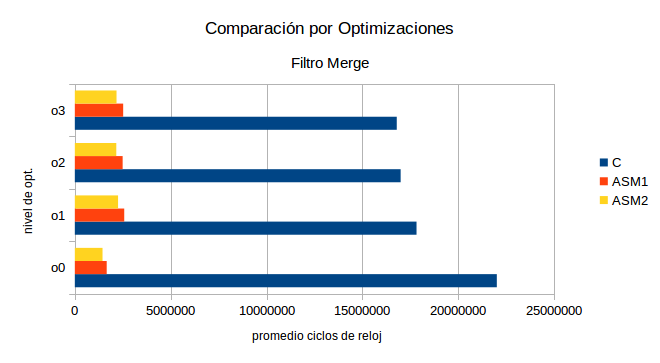
\includegraphics[width=125mm]{imagenes/resultados/grafico-opt-merge.png}
\caption{Filtro Merge, Experimento 3.}
\end{figure}

\begin{figure}[ht!]
\centering
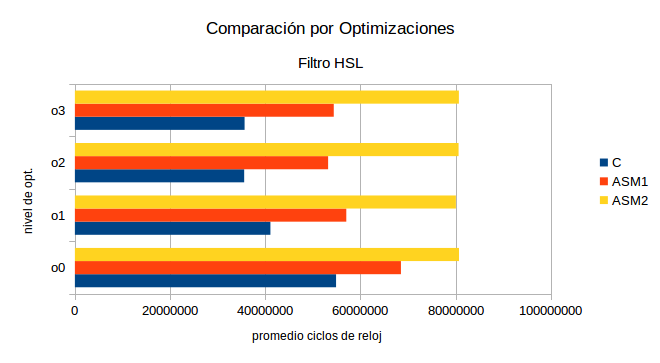
\includegraphics[width=125mm]{imagenes/resultados/grafico-opt-hsl.png}
\caption{Filtro HSL, Experimento 3.}
\end{figure}

\pagebreak
\pagebreak
\newpage

\subsection{Experimento 4}

En este experimento ejecutamos y comparamos las implementaciones con imágenes de distintos colores de fondo, siendo estos Rojo, Verde, Azul, Blanco y Negro.

\begin{figure}[ht!]
\centering
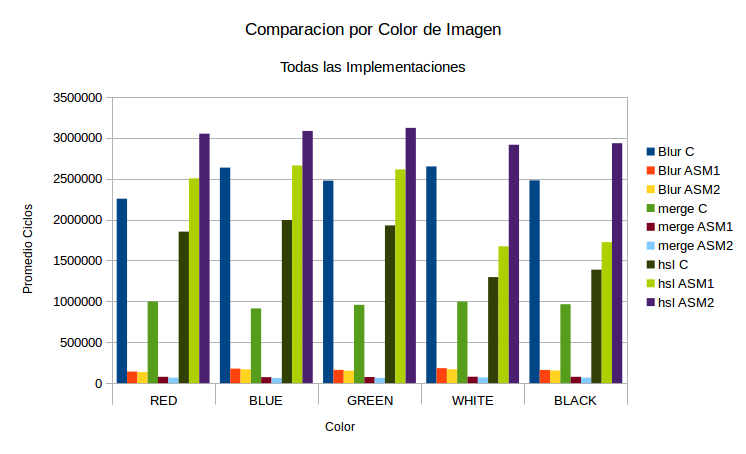
\includegraphics[width=120mm]{imagenes/resultados/grafico-colores1.png}
\caption{Comparación Filtros, Experimento 4.}
\end{figure}

Como se ve en la figura, en la mayoría de las implementaciones no se nota una diferencia importante, todas se comportan de manera similar, excepto HSL, que como se ve en detalle en la próxima figura, sus implementaciones de C y de ASM1 tardan menos con imágenes blancas o negras.

\begin{figure}[ht!]
\centering
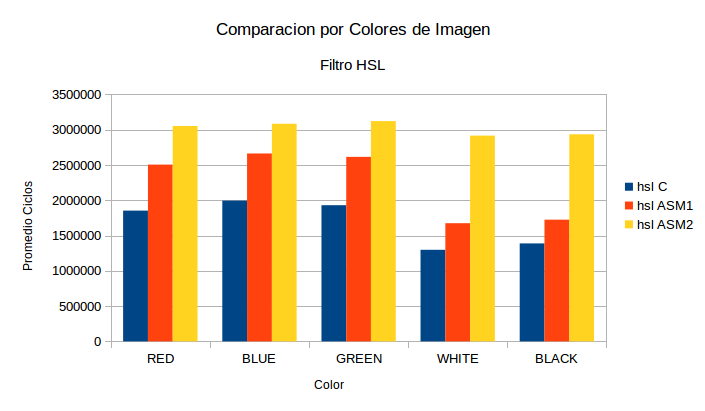
\includegraphics[width=110mm]{imagenes/resultados/grafico-colores2.png}
\caption{Comparación Filtros HSL, Experimento 4.}
\end{figure}

Ésto se debe a que para realizar las conversiones de rgb a hsl y viceversa, la complejidad del algoritmo para píxeles en blanco o negro se simplifica, ya que en ambos casos entrara en el primero de los ifs de las conversiones, sin necesidad de entrar a los else, mientras que en el ASM2 si debera ejecutar todas las ramas, reemplazando en caso de que sea necesario por el nuevo valor.
Como conclusión podemos sacar, que ASM2 corre con desventaja con respecto a ASM1 y C para todos los píxeles cuyas componentes coincidan en su valor, ya que en esos casos también se simplifica el cálculo para la conversión de un modelo a otro en la funcion de C. (Si los componentes son iguales, cmax==cmin , haciendo que el valor de h sea 0, y si al sumar queda menor de 60, cuando se convierta a RGB tambien alcanzara con el primer if, sin necesidad de ejecutar los otros).
Hay que tener en cuenta que por cada if, nuestra implementacion utiliza instrucciones de SHUFFLE, cuyos costos ifluyen directamente en el rendimiento de ASM2.

\newpage

\subsection{Experimento 5}


Como último experimento, decidimos analizar si podríamos optimizar los algoritmos reduciendo la cantidad de saltos condicionales. Para ello propusimos dos maneras de comprobar si esto valdría la pena. 
Las mediciones de este experimento se realizaron, por comodidad, sobre las implementaciones del filtro Merge.
Por un lado, medimos el promedio de 1000 iteraciones aplicando la función a dos imágenes de 32x32 y 1024x1 pixel respectivamente, de manera que ambas tienen la misma cantidad de píxeles, pero la segunda sólo entrará una vez al ciclo de filas.
Por otro lado, modificamos el algoritmo de manera que se recorra la imagen tan sólo en un ciclo, calculando la cantidad de iteraciones como el alto en píxeles de la imagen por el ancho de la imagen multiplicado por 4 (es decir, por el ancho en bytes de una fila de la imagen).

\begin{figure}[ht!]
\centering
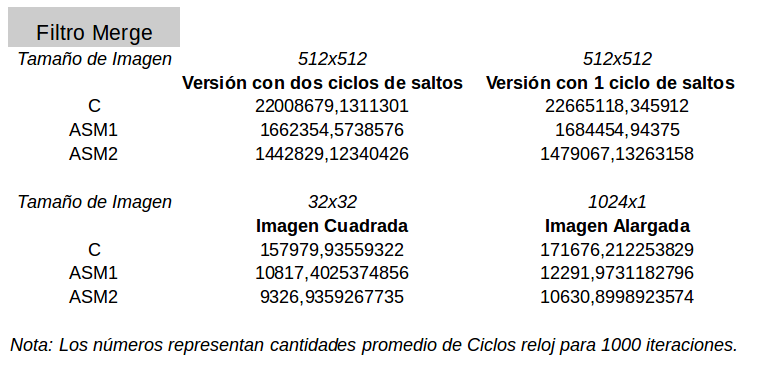
\includegraphics[width=130mm]{imagenes/resultados/tabla-saltos.png}
\caption{Resultados para Filtros Merge con menos saltos, Experimento 5.}
\end{figure}

Como se muestra en la tabla, en ambos casos no obtuvimos mejoras significativas, sino que se comportaban muy similar entre las dos. Con esto llegamos a la conclusión de que en imágenes relativamente pequeñas, utilizar 1 o 2 ciclos para recorrer la matriz no modifica la performance del algoritmo. Queda pendiente probar que sucede en mapas de bits realmente grandes, pero consideramos que estos filtros no trabajan sobre imagenes de tal tamaño.

